%\documentclass[12pt, oneside, a4paper, openany]{article}
\documentclass[14pt, oneside, a4paper, openany]{scrartcl}
\usepackage[utf8]{vietnam}
\usepackage{amsmath, amsbsy, amsxtra, latexsym, amssymb, inputenc}
\usepackage[top=3.5cm, bottom=3cm, left=3.5cm, right=2cm]{geometry}
\usepackage{times}
\usepackage{graphicx}
\usepackage{systeme}
\usepackage{multirow}
\usepackage{imakeidx}
\makeindex[options=-s index,columns=2,intoc=true]
\usepackage{indentfirst}
\setlength{\parindent}{1cm}
\usepackage{array}
\usepackage{hyperref}

% first page
\linespread{1.25}
\let\circledS\undefined
\mathchardef\period=\mathcode`,
\newtheorem{example}{Ví dụ}[section]
\newtheorem{definition}{Định nghĩa}[section]
\mathchardef\period=\mathcode`,
\begin{document}

\thispagestyle{empty}

\centerline{\bf TRƯỜNG ĐẠI HỌC BÁCH KHOA HÀ NỘI}
\centerline{\bf VIỆN TOÁN ỨNG DỤNG \& TIN HỌC}
\centerline{\bf--------------------o0o--------------------}
\vspace*{1cm}
\begin{figure}[!ht]
\centering

\includegraphics[height=4cm,width=3cm]{anhbia.jpg} 
\end{figure}
\vspace*{1cm}
\centerline{\Large\bf ỨNG DỤNG NHẬN DIỆN VÀ ĐẾM SỐ CÂY CỌ}
\centerline{\large\bf SỬ DỤNG PHƯƠNG PHÁP HAAR-BASED CASCADE CLASSIFIER}
\vspace*{1cm}
\centerline{\LARGE\bf ĐỒ ÁN 3}
\centerline{\Large\bf Chuyên ngành: Toán Tin}
\vspace*{2cm}

\hspace{1.95cm} \textbf{Giáo viên hướng dẫn } 
\hspace{4mm} \textbf{:}
\textbf{\parbox[t]{10cm}{\hspace{0.85cm}LÊ KIM THƯ}}

\hspace{2cm} \textbf{Sinh viên thực hiện }
\hspace{0.7cm} \textbf{:}
\textbf{\parbox[t]{10cm}{\hspace{0.85cm}NGÔ TRƯỜNG GIANG}}

\hspace*{1.95cm} \textbf{SHSV } 
\hspace{3.5cm} \textbf{:}
\hspace{10pt} \textbf{\parbox[t]{10cm}{\hspace{0.45cm}20121584}}
\vspace{2.5cm}
\vfill
\centerline{\bf Hà Nội - 06/2017}

\newpage
\thispagestyle{empty}
\centerline{\Large\bf NHẬN XÉT CỦA THẦY HƯỚNG DẪN}
\begin{enumerate}
	\item \textbf{Mục đích và nội dung của đồ án}
	\newline
	\newline
	\newline
	\newline
	\item \textbf{Kết quả đạt được}
	\newline
	\newline
	\newline
	\newline
	\item \textbf{Ý thức làm việc của sinh viên} \ldots
	\newline
	\newline
	\newline
	\newline
	\newline
	
	\begin{flushright}
		Hà Nội, ngày 05 tháng 05 năm 2017
	\end{flushright}
	\hspace{95 mm}Giảng viên hướng dẫn
	
	%\vspace*{2cm}
	\hspace{95 mm}(Ký và ghi rõ họ tên)
\end{enumerate}

%Create table of contents
\newpage
\thispagestyle{empty}
\tableofcontents
\newpage
% Create table of figures
\thispagestyle{empty}
\listoffigures
\listoftables
\newpage
\section{Lời cảm ơn}
Lời đầu tiên, em xin chân thành cảm ơn các thầy giáo trong Trường Đại học Bách Khoa Hà Nội, cùng các thầy cô trong Viện Toán ứng dụng và Tin học, đã dành tâm huyết truyền đạt những kiến thức quý báu cho chúng em trong suốt những năm tháng học em tại trường.

Với lòng biết ơn sâu sắc, em xin cảm ơn cô Lê Kim Thư đã giúp đỡ em rất nhiều trong quá trình thực hiện đồ án này.

Em cũng xin cảm ơn gia đình và bạn bè đã động viên, giúp đỡ em rất nhiều trong thời gian em làm đồ án.

Cuối cùng em xin chúc các thầy cô giáo trong Trường Đại Học Bách Khoa Hà Nội lời chúc sức khỏe và thành đạt.

\begin{flushright}
	Hà Nội, ngày 05 tháng 05 năm 2017
\end{flushright}
%\vspace*{2cm}
\hspace{95 mm}Ngô Trường Giang

\newpage
\section{Lời nói đầu}
Cây cọ dầu là loại cây công nghiệp có vai trò quan trọng trong kinh tế của đất nước nhiệt đới Malaysia, đất nước đứng thứ hai thế giới về sản lượng dầu cọ, với sản lượng năm 2014 đạt 19.5 tỉ tấn. Nguồn lợi kinh tế đem lại cho đất nước này từ ngành công nghiệp dầu cọ ước tính 16.1 tỉ USD vào năm 2015, chiếm 5-6\% GDP của cả đất nước này. 
Diện tích và sản lượng trồng cọ được kiểm soát bởi cả các hộ trồng cọ nhỏ lẻ (chiếm khoảng 40\%) và các công ty dầu cọ lớn (chiếm khoảng 60\%) (nguồn \href{http://cleanmalaysia.com/2015/12/09/just-how-big-is-malaysias-palm-oil-industry/}{cleanmalaysia} \cite{cleanmalay}).
Việc giám sát được quá trình phát triển, phát hiện ra những vùng trồng cọ mới và ước tính được sản lượng trồng cọ của mỗi vùng là một yếu tố quan trọng trong dự báo và kiểm soát giá của dầu cọ trên thị trường.

\begin{figure}[!h]
	\centering
	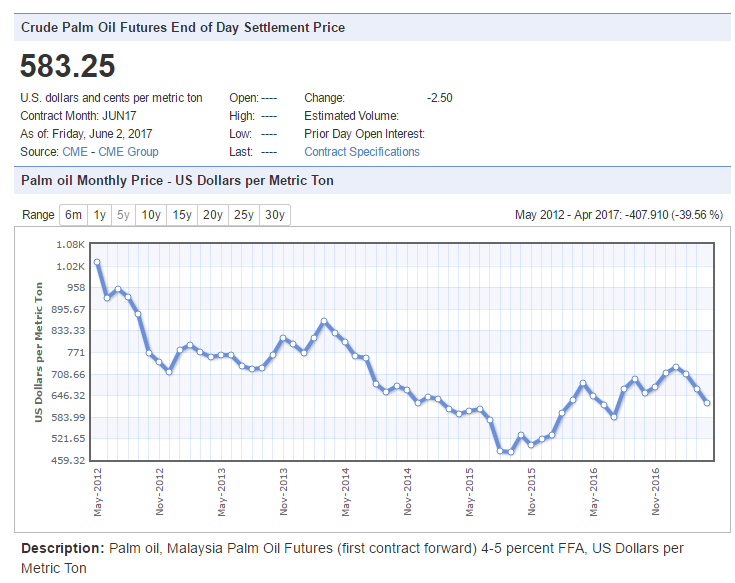
\includegraphics[scale=0.8]{figures/oilPalmMarket.png} 
	\caption[Tình hình thị trường dầu cọ trong 5 năm trở lại đây]{Tình hình thị trường dầu cọ trong 5 năm trở lại đây (nguồn \href{http://www.indexmundi.com/commodities/?commodity=palm-oil&months=60}{indexmundi}\cite{indexmundi})}
\end{figure}

Số cây cọ trong một vùng trồng cọ là một thông tin cơ bản để theo dõi được sự phát triển của cây cọ cũng như tính toán được sản lượng, bước đầu của nông nghiệp thông minh (intelligent agriculture).

Cùng với sự phát triển của khoa học viễn thám, ngành khoa học về thu thập thông tin về những đối tượng địa lý, từ trên cao, thường là vệ tinh hoặc máy bay. Dữ liệu ảnh độ phân giải cao về mặt đất đang càng ngày càng phổ biến.

Trong báo cáo này, tôi sẽ trình bày phương pháp sử dụng ảnh viễn thám của vùng Jalan Bukit Kuantan, Malaysia, giúp tự động nhận diện và đếm số lượng cây cọ có trong ảnh của một vùng trồng cọ dầu.

Phương pháp được sử dụng là phương pháp nhận diện đối tượng Haar-based Cascades Classifier, được đề xuất bởi P. Viola và M. Jones[1] năm 2001.

Tôi đã sử dụng phương pháp này để luyện một máy học trên tập dữ liệu ảnh cây cọ dầu thu được từ nguồn ảnh viễn thám ban đầu, từ đó tạo ra chương trình máy học có khả năng nhận diện và đếm số cây cọ với độ chính xác tương đối tốt. Thư viên xử lý ảnh mã nguồn mở OpenCV \href{http://opencv.org}{OpenCV} \cite{opencv} được tôi sử dụng để đào tạo máy học và nhận diện cây trong ảnh.
\newpage
\section{Giới thiệu và đặt vấn đề}
\subsection{Viễn thám, ảnh vệ tinh chất lượng cao, ảnh UAV}
Viễn thám \index{Viễn thám} là ngành khoa học về quan sát và thu thập thông tin về những đối tượng và hiện tượng diễn ra mà không liên hệ trực tiếp với đối tượng đó, do đó trái ngược với quan sát thực địa.

Viễn thám được sử dụng trong rất nhiều lĩnh vực khác nhau, gồm có địa lý, những ngành trong khoa học trái đất (ví dụ như sinh thái học, thủy văn học, hải dương học, địa chất học,v.v.), và cả trong quân sự, kinh tế, và nhiều ngành khác nữa.
Gần đây, khái niệm viễn thám thường được sử dụng để nhắc đến việc sử dụng các vệ tinh hoặc máy bay cùng với các công nghệ cảm biến hiện đại nằm nhận diện và phân loại các vật thể trên trái đất, sử dụng các loại tín hiệu điện từ.

Viễn thám có thể chia ra hai loại chính là viễn thám chủ động (tín hiệu được phát ra từ vệ tinh hoặc máy bay và bị phản xạ ngược trở lại hoặc bị hấp thu bởi các đối tượng, thu lại được bằng các cảm biến) và viễn thám bị động (thu nhận sự phản chiếu ánh sáng mặt trời từ các vật thể vào các cảm biến) (nguồn \href{https://en.wikipedia.org/wiki/Remote_sensing}{Wikipedia})\cite{remotesens}.
Chất lượng của ảnh vệ tinh được quyết định bởi các độ phân giải sau:
\begin{itemize}
	\item Độ phân giải không gian, kích thước của một pixel được ghi lại trong ảnh vệ tinh ứng với bao nhiêu mét trên thực địa.
	\item Độ phân giải phổ, số bước sóng của những giải tần số khác nhau tạo ra những băng khác nhau được ghi lại trong ảnh viễn thám.
	\item Độ phân giải giá trị thu được, khi số hóa các giá trị thu được bằng cảm biến, thường nằm trong phạm vi từ 8 cho tới 16 bit trong ảnh viễn thám.
	\item Độ phân giải thời gian là tần suất bay qua và thu được thông tin về một khu vực nhất định của vệ tinh hoặc máy bay và được sử dụng trong phân tích chuối thời gian.
\end{itemize}
Trong những năm gần đây, công nghệ cảm biến và khoa học hàng không vũ trụ đã phát triên mạnh mẽ, trở thành một ngành công nghiệp chứ không còn là độc quyền của chính phủ các nước. Kết quả của sự phát triển này là thu được ảnh vệ tinh chất lượng cao  \index{ảnh vệ tinh chất lượng cao} (very high resolution - VHR) với độ phân giải không gian nhỏ hơn 1m, đã được thu thập phủ khắp bề mặt trái đất, nổi bật là những vệ tinh mới như \href{http://www.satimagingcorp.com/gallery/geoeye-1/}{GeoEye-1} \cite{geoeye} và các vệ tinh WorldView-1,WorldView-2,WorldView-3 và WorldView-4 của \href{https://www.digitalglobe.com/}{DigitalGlobe} \cite{digiglob}.

Những ảnh vệ tinh chất lượng cao đã đóng góp lớn trong công nghệ viễn thám hiện đại, khi mang đến ảnh chất lượng tốt hơn, các độ phân giải cao hơn, đa dạng thông tin hơn về trái đất, giúp người sử dụng ảnh đưa ra quyết định chính xác, cũng như góp phần xây dựng bản đồ thế giới đầy đủ hơn.

Bên cạnh ảnh vệ tinh chất lượng cao, ảnh của thiết bị bay không người lái \index{ảnh của thiết bị bay không người lái} (unmanned aerial vehicle - UAV) cũng đang được sử dụng bởi cộng đồng viễn thám như một hệ thống thu thập dữ liệu thông tin địa lý mới không kém phần hiệu quả.

Trong một thời gian dài trước đây, ảnh UAV chỉ được sử dụng cho mục đích quân sự, nhưng với sự tiến bộ của công nghệ và giá thành giảm, những thiết bị bay không người lái trở thành một giải pháp thực tiễn cho nhiều ứng dụng khác nhau như giám sát nông nghiệp, phát hiện thay đổi bất thường, nông nghiệp chính xác hay đếm xe ôtô.

Tính linh động cao của những thiết bị UAV cho phép sự can thiệp ngay lập tức và đo lường có tương tác theo những yêu cầu cụ thể của khách hàng.

Trong thực tế, UAV có khả năng:
\begin{enumerate}
	\item Cho phép theo giõi một vùng diện tích nhỏ với độ phân giải không gian cực nhỏ (lên đến $1cm$/pixel).
	\item Có thể di chuyển đến điểm mong muốn theo giõi chỉ trong vài phút.
	\item Cho phép thu thập thông tin theo chiều thời gian của cùng một vùng tại những khoảng thời gian xác định.
\end{enumerate}

Tuy nhiên, ảnh UAV cũng gặp phải những khó khăn khi những phương pháp xử lý ảnh từng được áp dụng cho ảnh vệ tinh trước đây không còn phù hợp nữa, vì những ảnh UAV có độ phân giải không gian nhỏ hơn nhiều.

%Trong báo cáo này, tôi sẽ trình bày phương pháp để nhận diện và đếm số cây cọ dầu trong ảnh viễn thám của vùng trồng cọ Kuantan, Malaysia.
\subsection{Máy học cơ bản và ứng dụng trong thị giác máy tính}
Theo \href{https://vi.wikipedia.org/wiki/H\%E1\%BB\%8Dc_m\%C3\%A1y}{Wikipedia}, \textbf{Máy học} \index{Máy học} (machine learning) là một lĩnh vực của trí tuệ nhân tạo (artificial intelligence) liên quan đến việc nghiên cứu và xây dựng các kĩ thuật cho phép các hệ thống "học" tự động từ dữ liệu để giải quyết những vấn đề cụ thể.

Máy học đã được ứng dụng không chỉ vào đời sống mà còn vào rất nhiều những lĩnh vực khoa học khác, một trong số đó chính là thị giác máy tính.

Thị giác máy tính \index{Thị giác máy tính} là một lĩnh vực liên ngành, quan tâm đến việc giúp máy tính đạt được khả năng hiểu được ảnh và video kĩ thuật số, từ đó trích xuất những thông tin hữu ích. Từ quan điểm kĩ thuật, thị giác máy tính tìm kiếm sự tự động hóa những tác vụ mà hệ thống thị giác của mắt người có thể làm được.

Một số tác vụ thông thường của hệ thống thị giác máy tính: nhân diện, phân tích chuyển động, khôi phục ảnh và tái tạo khung cảnh.

Nhận diện đối tượng là một hướng lớn và được tập trung rất nhiều trong thị giác máy tính, đồng thời những kĩ thuật máy học được tạo ra để phục vụ cho tác vụ này cũng rất phong phú. Trong nhận diện đối tượng thì nhiệm vụ cơ bản là xác định được vị trí của một loại đối tượng cần tìm ở trong ảnh. Nếu có nhiều đối tượng thuộc loại đó xuất hiện thì cũng phải tìm được vị trí của tất cả các đối tượng này.

Bài toán đếm số cây cọ có thể đưa về bài toán nhận diện cây cọ trong ảnh và sử dụng phương pháp máy học để nhận diện là có cây cọ trong ảnh hay không, kêt hợp với phương pháp tìm kiếm đối tượng trong ảnh thường được sử dụng, là phương pháp cửa sổ trượt \index{phương pháp cửa sổ trượt} (slicing window) để nhận diện tất cả số cây cọ có trong ảnh. 
Trong phương pháp cửa sổ trượt, mỗi cửa sổ là một khung hình kích thước cho trước, nhỏ hơn kích thước của ảnh, trượt đi theo chiều dọc và chiều ngang của anh đến khắp các vị trí trong ảnh. Những ảnh con thu được bằng việc cắt ảnh gốc sử dụng cửa sổ này khi trượt qua mỗi vị trí sẽ được đưa vào máy học nhận diện đối tượng. Máy học nhận diện đối tượng lúc này là một phân lớp nhị phân, trong đó đầu ra của máy học chỉ là có hay không có cây cọ ở trong ảnh. Khi một cửa số đã duyệt hết bức ảnh, ta có thể thay đổi kích thước cửa sổ và thực hiện duyệt lại lần nữa để tìm kiếm những đối tượng có kích thước nhỏ hơn hoặc lớn hơn.

\begin{figure}
	\centering
	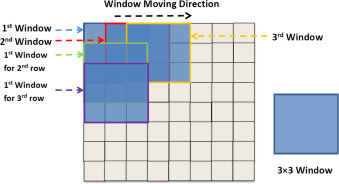
\includegraphics[scale=1]{figures/slicingWindow.jpg} 
	\caption[Kĩ thuật cửa sổ trượt]{Kĩ thuật cửa sổ trượt trong nhận diện đối tượng.}
\end{figure}


\subsection{Ứng dụng xử lý ảnh viễn thám vào nhận diện cây cọ dầu}
Cọ dầu là cây công nghiệp phát triển trong vùng khí hậu nóng ẩm. Dầu cọ được chiết xuất từ thịt của quả cây cọ dầu trở thành nguyên liệu thô cho rất nhiều sản phẩm mà đứng đầu là dầu ăn vì sản lượng của dầu cọ rất lớn so với các loại cây cho dầu khác như hướng dương, đậu nành hay cải dầu. 

Dầu cọ có nhu cầu rất lớn trên thị trường khiến cho sự phát triển của diện tích trồng cọ đã tăng trưởng nhanh chóng trong vài thập kỉ gần đây.

Trong báo cáo này, tôi sẽ trình bày phương pháp đếm số cây cọ trong ảnh viễn thám từ dữ liệu ảnh vệ tinh chất lượng cao chụp một vùng trồng cọ ở thành phố Kuantan, Malaysia. 

Ảnh vệ tinh chất lượng cao sau khi được tiền xử lý, sẽ được dùng để lấy mẫu những ảnh con chứa cây cọ dầu và những ảnh con không chứa cây cọ dầu. Những ảnh mẫu được tạo ra từ quá trình tiền xử lý và lấy mẫu sẽ được dùng để luyện máy học giúp tự động nhận diện và đếm số cây cọ dầu có ở trong ảnh.

Với phương pháp nhận diện đối tượng Haar-based Cascade Classifier được đề xuất bởi P. Viola và M. Jones [1], máy học thu được bằng cách áp dụng phương pháp này trong có khả năng đếm nhanh chóng số lượng cây cọ dầu trong ảnh.

Cuối cùng, tôi sẽ trình bày một ứng dụng desktop, sử dụng thư viện OpenCV và ngôn ngữ lập trình Python, thực thi phương pháp nhận diện đối tượng Haar Cascade, để đếm số cây cọ có trong một bức ảnh viễn thám khác của vùng khác thuộc Kuantan, Malaysia.

\newpage
\section{Phương pháp thực hiện}
Sau đây, tôi sẽ trình bày phương pháp học máy được sử dụng trong bài này để nhận diện và đếm số cây cọ dầu trong ảnh viễn thám, phương pháp Haar-Based Cascade Classifier do  P. Viola và M. Jones[1] đề xuất.
\subsection{Phương pháp nhận diện đối tượng Haar Cascade}
\subsubsection{Đặc trưng dạng Haar và ảnh nguyên (Integral Image)}
Thủ tục nhận diện đối tượng ở trong một bức ảnh phụ thuộc vào giá trị thu được của những đặc trưng thu được từ ảnh đó. Có rất nhiều lý do cho việc sử dụng đặc trưng thay vì từng pixel ảnh. Lý do chung nhất là những đặc trưng này có khả năng mã hóa những tri thức học được từ tập dữ liệu luyên. Lý do thứ hai là hệ thống phân lớp dựa trên đặc trưng thì nhanh hơn dựa trên từng pixel.
Những đặc trưng dạng Haar là những đặc trưng của ảnh kỹ thuật số, có cái tên bắt nguồn từ sự tương tự với Haar wavelet[?], và là một trong những đặc trưng được sử dụng phổ biến trong nhận dạng đối tượng.

Papageorgiou et al.[?] đã đề cập đến việc sử dụng những đặc trưng dựa trên Haar wavelets thay vì sử dụng cường độ sáng tại mỗi điểm ảnh. Viola và Jones đã sử dụng ý tưởng này và phát triển những đặc trưng dạng Haar (Haar-like features).
Một đặc trưng dạng Haar tính toán trên những vùng hình chữ nhật kề nhau tại một vị trí xác định trên cửa số nhận diện, tính tổng cường độ sáng (giá trị tại mỗi pixel trong ảnh grayscale) trong mỗi vùng và tính hiệu của những tổng này.
Ví dụ, ta có một cơ sở dữ liệu hình ảnh về mặt người. Dễ dàng quan sát thấy trong tất cả các ảnh rằng vùng mắt thường tối hơn so với vùng má. Do đó một đặc trưng dạng Haar cho mặt người có thể là hai hình chữ nhật kề nhau nằm trên vùng mắt và vùng má. Vị trí của hai hình chữ nhật này được định nghĩa tương đối với cửa sổ nhận diện.

\begin{figure}
	\centering
	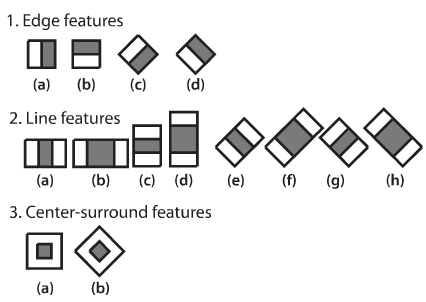
\includegraphics[scale=0.8]{figures/HaarFeatures.png} 
	\caption[Một số đặc trưng dạng Haar cơ bản]{Một số đặc trưng dạng Haar cơ bản, (1) Các đặc trưng 2 hình chữ nhật, 
		(2) Các đặc trưng 3 hình chữ nhật,
		(3) Các đặc trưng dạng trung tâm.}
\end{figure}

Để tính toán tổng cường độ sáng trong một hình chữ nhật nhanh chóng, Viola và Jones[1] đã sử dụng một dạng biểu diễn trung gian cho ảnh được gọi là ảnh nguyên (integral image). Ảnh nguyên có cùng kích thước với ảnh thực, giá trị của ảnh nguyên tại mỗi điểm ảnh $(x,y)$ bao gồm tổng cường độ sáng của số pixel nằm về phía bên trái và phía trên của $(x,y)$. Công thức tính giá trị ảnh nguyên:
$$
ii(x,y) = \sum_{x' \leq x, y' \leq y} i(x',y')
$$
Với $ii(x,y)$ là ảnh nguyên và $i(x,y)$ là ảnh gốc.
\begin{figure}
	\centering
	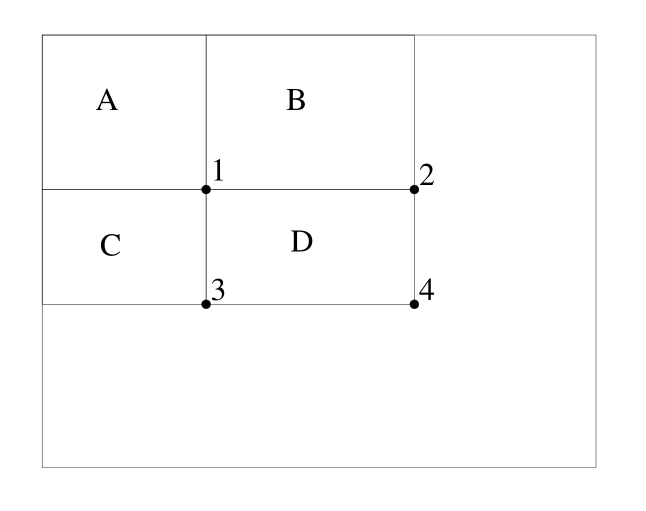
\includegraphics[scale=0.5]{figures/integralImage.png} 
	\caption[Tổng cường độ sáng trong hình chữ nhật]{Tổng cường độ sáng trong hình chữ nhật D được tính bằng $ii(4) + ii(1) - ii(2) - ii(3)$}
\end{figure}
Sử dụng ảnh nguyên, bất kì hình chữ nhật có cũng có thể tính tổng cường độ sáng nhanh bằng 4 giá trị của ảnh nguyên tại 4 đỉnh của hình chữ nhật, thời gian tính toán là hằng số. Đây cũng chính là ưu điểm của đặc trưng dạng Haar so với các đặc trưng khác, thời gian tính toán rất nhanh.

\subsubsection{Nhận xét}
Những đặc trưng dạng Haar chỉ giới hạn trong các hình chữ nhật, và chỉ có 3 hướng cơ bản: dọc, ngang và chéo $45^o$, nên những đặc trưng này thường rất yếu trong nhận diện ảnh. Tuy nhiện, tập hợp của những đặc trưng này, lại cung cấp một sự thể hiện tốt của đối tượng cần nhận diện.

Với độ phân giải của cửa số nhận diện là $24$x$24$, số lượng đặc trưng dạng Haar cũng đã khá lớn, lên đến hơn $180,000$ đặc trưng. Đa phần trong số chúng là không có ý nghĩa. Mặc dù các đặc trưng có thể tính toán rất nhanh, tính toán trên tập tất cả đặc trưng này vẫn rất tốn thời gian. Giả thiết dược Viola và Jones[1] đặt ra bằng thực nghiệm là chỉ có một số lượng rất ít trong số những đặc trưng này có thể kết hợp để tạo ra một máy học phân lớp hiệu quả. Do đó, ta cần lựa chọn ra những đặc trưng hiệu quả trong nhận diện đối tượng và xây dựng một máy học phân lớp dựa trên tập những đặc trưng hiệu quả này.

\subsubsection{Phương pháp xây dựng máy học phân lớp dựa trên AdaBoost}
Cho một tập những đặc trưng và một tập dữ liệu luyện được gán nhãn dương (có đối tượng cần nhận diện) và âm (không có đối tượng cần nhận diện), bất kỳ phương pháp máy học phân lớp nào cũng có thể dùng để học hàm phân lớp hai loại dữ liệu này. Viola và Jones[1] đã lựa chọn một phương pháp tương tự như AdaBoost để lựa chọn ra một tập nhỏ những đặc trưng và luyện một máy học phân lớp.

Thuật toán ở đây được thiết kế để lựa chọn ra những đặc trưng tốt nhất cho việc phân lớp những ảnh dương và âm.
Cho mỗi đặc trưng, một hàm ngưỡng phân lớp tối ưu được lựa chọn để tối thiểu hóa số ảnh bị phân nhầm lớp. Hàm phân lớp này kí hiệu là $h_j(x)$ của đặc trưng $f_j$, với ngưỡng $\theta_j$ và parity $p_j$ để chỉ chiều của bất phương trình, có dạng:
$$
h_j(x)=
\begin{cases}
	1& \text{nếu $p_j f_j(x) < p_j\theta_j$},\\
	0& \text{ngược lại}.
\end{cases}
$$
Ở đây $x$ là một cửa sổ kích thước $24x24$ của ảnh.

Sơ đồ của quá trình boosting được trình bày trong bảng 1.

\begin{table}
\caption[Thuật toán AdaBoost cho học phân lớp]{Thuật toán AdaBoost cho học phân lớp. Mỗi vòng lặp lựa chọn ra một đặc trưng từ danh sách những đặc trưng.}
\begin{tabular}{ |m{15cm}| } 
	\hline
	\begin{itemize}
		\item Cho một tập ảnh mẫu $(x_1,y_1),...,(x_n,y_n)$ với $y_i=0,1$ ứng với mẫu là âm (không chứa đối tượng cần nhận diện) hay dương (có chứa đối tượng cần nhận diện).
		\item Khởi tạo các trọng số $w_{1,i}= \frac{1}{2m}$ với $y_i=0$ và $w_{1,i}= \frac{1}{2l}$ với $y_i=1$, trong đó $m$ và $l$ lần lượt là số mẫu dương và mẫu âm.
		\item For $t = 1,...,T$:
		\begin{enumerate}
			\item Chuẩn hóa những trọng số:
			$$
			w_{t,i} \rightarrow \frac{w_{t,i}}{\sum_{j=1}^{n}w_{t,j}}
			$$
			sao cho  vectơ trọng số $w_t$ là phân phối xác suất.
			\item với mỗi đặc trưng, j, luyện một hàm phân lớp $h_j$. Tỉ lệ lỗi được tính ứng với $w_t$,
			$$
			\epsilon_j = \sum_i w_j|h_j(x_i) - y_i|
			$$
			\item Chọn một hàm phân lớp $h_t$ với tỉ lệ lỗi thấp nhất $\epsilon_t$
			\item cập nhật các trọng số:
			$$
			w_{t+1,i} = w_{t,i} \beta_t^{(1-e_i)}
			$$
			trong đó $e_i=0$ nếu $x_i$ được phân lớp đúng, $e_i=1$ nếu ngược lại, và $\beta_t = \frac{\epsilon_t}{1 - \epsilon_t}.$
		\end{enumerate}
		\item Hàm phân lớp cuối cùng được tính dựa trên các $h_t$ được lựa chọn ra:
		$$
		h(x)=
		\begin{cases}
			1& \text{nếu $\sum_{t=1}^{T}\alpha_t h_t(x) \geq \frac{1}{2}\sum_{t=1}^{T}\alpha_t$},\\
			0& \text{ngược lại}.
		\end{cases}
		$$
		với $\alpha_t = \log\frac{1}{\beta_t}$
	\end{itemize}
	\\
	\hline
\end{tabular}
\end{table}

\subsubsection{Phương pháp xây dựng máy học phân lớp hiệu quả dạng Cascade}
Phần này sẽ mô tả một thuật toán xây dựng một máy học phân lớp dạng thang cascade hay dạng tầng, để tăng hiệu năng của quá trình nhận diện đồng thời giảm thời gian tính toán.

Trước hết ta nhắc đến một số khái niệm trong phân lớp nhị phân được sử dụng ở phần này.

Giả sử gọi hàm phân lớp nhị phân là hàm $f(x)$ và ngưỡng của phân lớp là $t$. khi $f(x) > t$, dữ liệu đầu vào $x$ được phân vào lớp dương, ngược lại $x$ được phân vào lớp âm.

Trong phân lớp nhị phân (binary classification), khi phân lớp một tập dữ liệu, hàm phân lớp được sử dụng cùng với một ngưỡng (threshold) được xác định để phân lớp. Hai lớp trong phân lớp nhị phân tường được gọi là lớp âm (negative) và lớp dương (positive). Trong nhận diện đối tượng, lớp dương thường là tập những đối tượng cần nhận diện, còn lớp âm thường là tập những đối tượng không phải đối tượng cần nhận diện.

Tùy vào cách lựa chọn ngưỡng $t$ mà ta thu được kết quả phân lớp với các đo lường về độ chính xác khác nhau. Một số khái niệm được định nghĩa dựa trên phân lớp nhị phân:
\begin{itemize}
	\item Một dữ liệu được gọi là True Positive (TP) nếu nó là dữ liệu dương và được nhận diện là thuộc lớp dương.
	\item Một dữ liệu được gọi là True Negative (TN) nếu nó là dữ liệu âm và được nhận diện là thuộc lớp âm.
	\item Một dữ liệu được gọi là False Postive (FP) nếu nó là dữ liệu âm nhưng đựng nhận diện thuộc lớp dương.
	\item Một dữ liệu được gọi là False Negative (FN) nếu nó là dữ liệu dương nhưng được nhận diện thuộc lớp âm.
\end{itemize}
Các tỉ lệ True Positive, True Negative, False Postive và False Negative được tính như sau:

tỉ lệ true positive (true positive rate):
\begin{equation}
	 TPR = \frac{TP}{TP + FN}
\end{equation}

Tỉ lệ true negative ( true negative rate):
\begin{equation}
	TNR = \frac{TN}{TN + FP}
\end{equation}

Tỉ lệ false negative ( false negative rate):
\begin{equation}
FNR = \frac{FN}{FN + TP}
\end{equation}

Tỉ lệ false positive ( false positive rate):
\begin{equation}
FPR = \frac{FP}{FP + TN}
\end{equation}

\begin{figure}[!h]
	\centering
	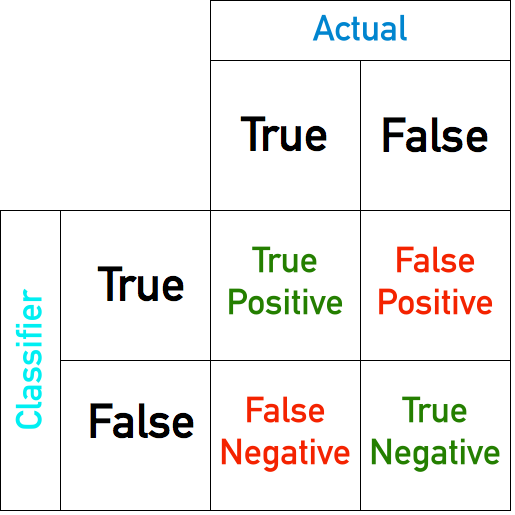
\includegraphics[scale=0.5]{figures/binaryclassifier.png} 
	\caption[Mô tả các kết quả của phân lớp nhị phân]{Mô tả các kết quả của phân lớp nhị phân.}
\end{figure}

Ý tưởng của phân lớp dạng cascade là sử dụng những máy học phân lớp đơn giản được xây dựng để loại bỏ phần lớn những cửa sổ âm (tỉ lệ false negative gần tới 0), trước khi sử dụng những máy học phân lớp phức tạp để đạt được tỉ lệ false positive thấp (loại bỏ những cửa sổ âm bị nhận diện là đối tượng).

Ngưỡng của một máy học phân lớp có thể điều chỉnh để đạt được tỉ lệ false negative gần tới 0, để đảm bảo không có cửa sổ nào có đối tượng bị bỏ sót, hoặc ngược lại, loại bỏ đi đa phần nhưng cửa sổ âm.

Dạng tổng quát của quá trình nhận dạng là một dạng đơn giản của cây quyết định, mà ta gọi là cascade. Những kết quả dương từ máy học phân lớp đầu tiên sẽ được đưa vào máy học phân lớp thứ hai và tiếp tục phân lớp. Kết quả dương của máy học phân lớp thứ hai sẽ được đưa vào máy học thứ ba, cứ thế tiếp diễn. Những cửa sổ bị các máy học phân lớp nhận diện là âm sẽ ngay lập tức bị loại bỏ khỏi lần phân lớp tiếp theo.

\begin{figure}[!h]
	\centering
	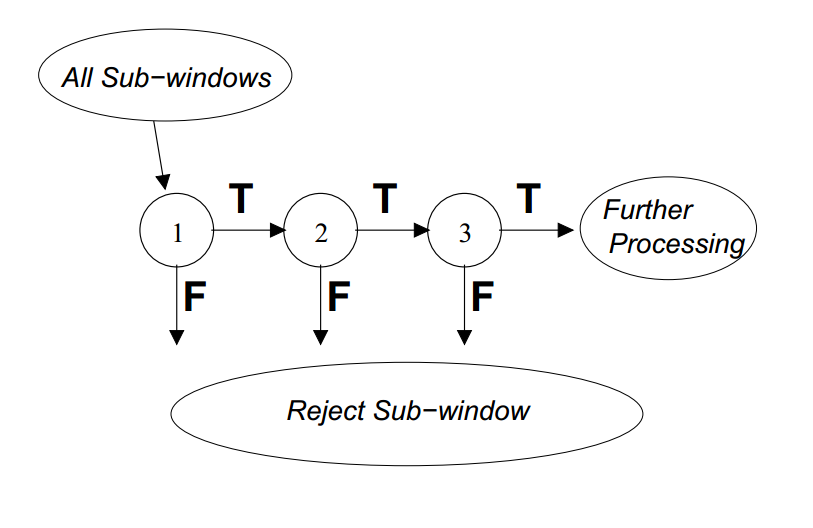
\includegraphics[scale=0.5]{figures/cascadeDetection.png} 
	\caption[Mô tả của một máy học nhận diện dạng cascade]{Mô tả của một máy học nhận diện dạng cascade. Một chuối những máy học phân lớp được áp dụng cho những cửa sổ. Máy học phân lớp đầu tiên sẽ loại bỏ một số lượng lớn những ví dụ âm với xử lý rất đơn giản (chỉ có một vài đặc trưng được sử dụng). Những máy học phân lớp tiếp theo sẽ loại bỏ những cửa sổ âm khác nhưng phức tạp hơn (nhiều đặc trưng hơn). Sau một vào bước xử lý, số cửa sổ phải xử lý giảm đi đáng kể. Phần cuối là xử lý về sau, có thể sử dụng một hệ thống nhận diện khác hoặc tiếp tục thêm các máy học phân lớp vào.}
\end{figure}
Cấu trúc của máy học nhận dạng cascade phản ánh thực tế rằng trong một bức ảnh, đa phần cửa số là âm, vì thế nó cố gắng loại bỏ những cửa sổ âm này ở những giai đoạn sớm nhất có thể, những cửa sổ dương sẽ được phân lớp dương lần lượt qua các mọi máy học phân lớp của cascade, sự kiện này hiếm khi xảy ra.

Luyện một máy học phân lớp dạng cascade liên quan đến sự đánh đổi. Trong hầu hết các trường hợp, nhiều đặc trưng được sử dụng hơn sẽ giúp đạt được tỉ lệ nhận diện cao hơn và tỉ lệ false positive thấp hơn. Đồng thời máy học phân lớp có nhiều đặc trưng sẽ tốn nhiều thời gian để tính toán hơn. Khi luyện một máy học phân lớp dạng cascade, ta quan tâm đến: 1. số máy học phân lớp, 2. số đặc trưng trong mỗi máy học, 3. ngưỡng của mỗi máy học, được điều chỉnh để tối thiểu hóa số đặc trưng cần tính toán nhưng vẫn đảm bảo độ chính xác yêu cầu.

Trong thực tế, một framework rất đơn giản được sử dụng để tạo ra một máy học phân lớp có hiệu năng cao. % Đó là tại mỗi giai đoạn, giảm tỉ lệ false positive và giảm tỉ lệ nhân diện.

Mỗi một giai đoạn (stage) của máy học casade được luyện bằng cách thêm vào những đặc trưng vào máy học giai đoạn này cho đến khi tỉ lệ nhận diện vào tỉ lệ false positive đạt được yêu cầu. Các giai đoạn được thêm vào cho tới khi tỉ lệ false positive và tỉ lệ nhận diện tổng thể đạt yêu cầu.

\newpage
\section{Kết quả thực hiện}
\subsection{Vùng ngiên cứu và dữ liệu}
Dữ liệu được sử dụng trong báo cáo này là hai ảnh được chụp bởi máy bay không người lái (UAV), chụp một vùng trồng cọ thuộc vùng Jalan Bukit Kuantan, Malaysia tại hai địa điểm khác nhau.
\begin{figure}[!h]
	\centering
	\begin{minipage}{0.45\textwidth}
		\centering
		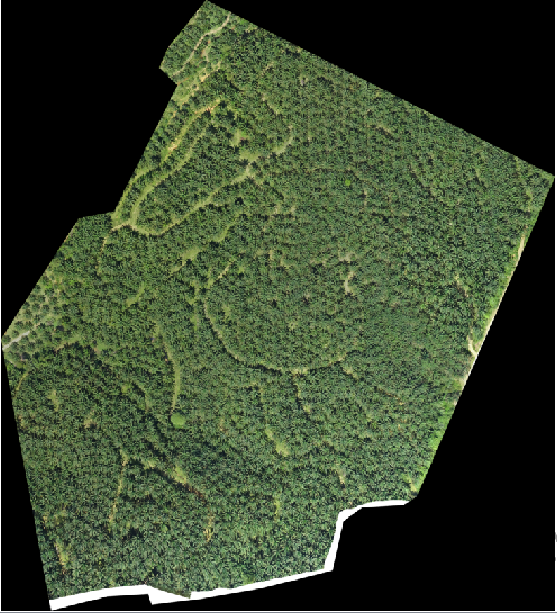
\includegraphics[width=0.9\textwidth]{figures/data02.png} % first figure itself
		\caption[ảnh vùng trồng cọ thứ nhất]{ảnh vùng trồng cọ thứ nhất, được sử dụng để làm dữ liệu luyện máy học nhận dạng cây cọ}
	\end{minipage}\hfill
	\begin{minipage}{0.45\textwidth}
		\centering
		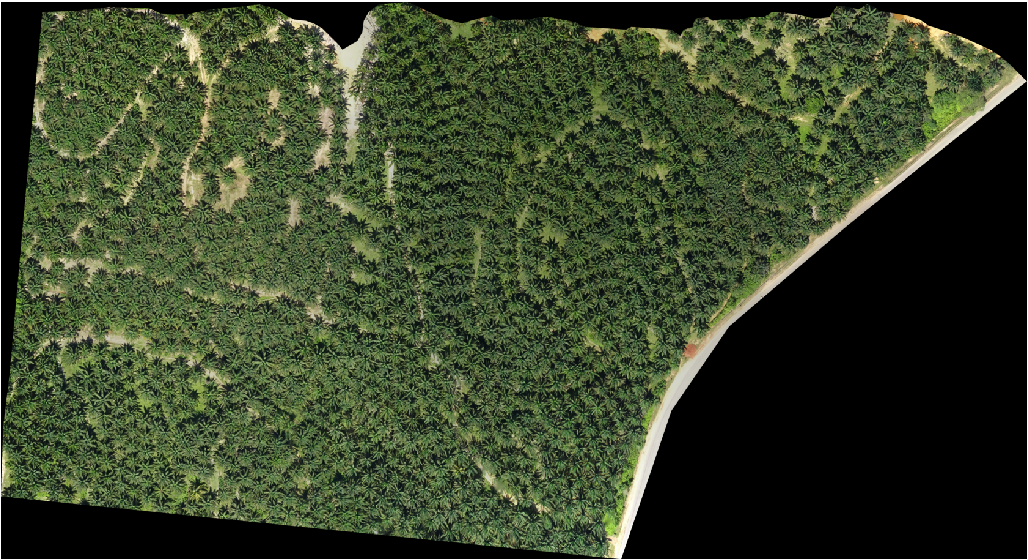
\includegraphics[width=0.9\textwidth]{figures/data01.png} % second figure itself
		\caption[ảnh vùng trồng cọ thứ hai]{ảnh vùng trồng cọ thứ hai, được sử dụng để làm dữ liệu kiểm tra độ chính xác của máy học nhận dạng}
	\end{minipage}
\end{figure}

\subsection{Sử dụng thư viện OpenCV để luyện máy học nhận diện và đếm cây cọ}
Trong bộ thư viện mã nguồn ở OpenCV đã có sẵn chương trình để luyện máy học phân lớp dạng cascade, được sử dụng để nhận dạng mặt người như một ví dụ áp dụng lý thuyết mà Viola Jones đã đề xuất.

Tôi đã sử dụng lại chương trình này, chạy với bộ dữ liệu cây cọ dầu thu thập được, thu được một máy học có khả năng nhận diện và đếm số cây cọ dầu có trong ảnh.

Sau đây là các bước của quá trình luyện máy học nhận diện cây cọ dầu:
\begin{enumerate}
	\item Chuẩn bị dữ liệu. Tại bước này, tôi sử dụng công cụ mã nguồn mở \href{http://www.qgis.org/en/site/}{QGIS} \cite{qgis} để thao tác trên dữ liệu thông tin địa lý, trích xuất ra ảnh những cây cọ từ ảnh của cả vùng trồng cọ.
	\begin{itemize}
		\item Bằng mắt, tôi chấm các điểm trên giao diện của QGIS, mỗi điểm này ứng với tâm của một cây cọ, đồng thời mỗi điểm được lưu dưới dạng tọa độ địa lý của điểm đó trên bản đồ.
		\item Tập những điểm này được lưu lại dưới dạng file \href{http://doc.arcgis.com/en/arcgis-online/reference/shapefiles.htm}{Shapefile} \cite{Shapefiles}, một định dạng lưu dữ liệu thông tin địa lý dạng vectơ, cụ thể ở đây là các điểm ứng với các tọa độ địa lý.
		\item Bằng ngôn ngữ lập trình \href{https://www.python.org/}{Python} \cite{python} và thư viện xử lý dữ liệu địa lý vectơ và ảnh viễn thám \href{http://gdal.org/}{GDAL} \cite{gdal}, tôi viết mã xử lý file shapefile đã tạo ra, trích lấy tọa độ các điểm trong file này, chuyển các điểm này sang hệ tọa độ của bức ảnh viễn thám, lựa chọn lấy một khung hình kích thước 80x80 lấy điểm này làm tâm, cắt ảnh nằm trong khung hình đó ra, lưu lại dưới dạng file ảnh. Thực hiện thao tác này với từng điểm trong file shapefile để thu được danh sách những ảnh chứa cây cọ để làm mẫu dương.
	\end{itemize}
	Lặp lại các bước trên, nhưng lựa chọn các vùng không phải là cây cọ, ta thu được tập dữ liệu ảnh mẫu âm.
	\begin{figure}[!h]
		\centering
		\begin{minipage}{0.5\textwidth}
			\centering
			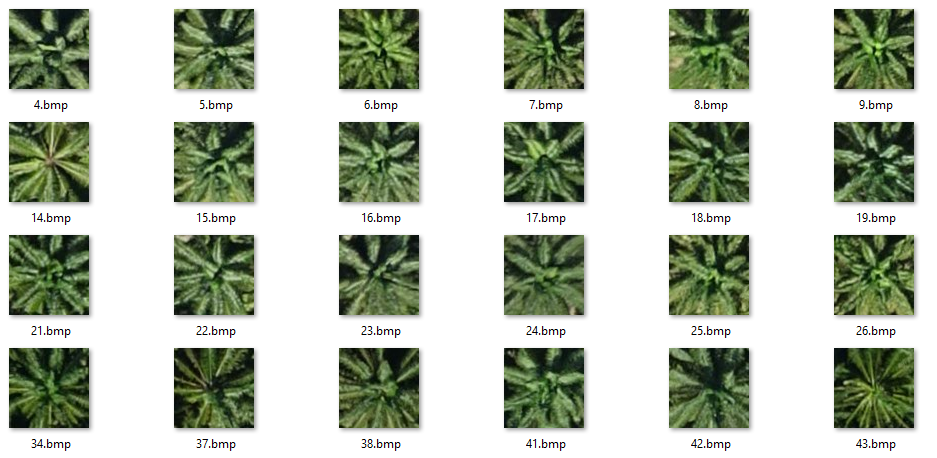
\includegraphics[width=0.9\textwidth]{figures/positiveList.png} % first figure itself
			\caption[Tập ảnh mẫu dương]{Tập ảnh mẫu dương}
		\end{minipage}\hfill
		\begin{minipage}{0.5\textwidth}
			\centering
			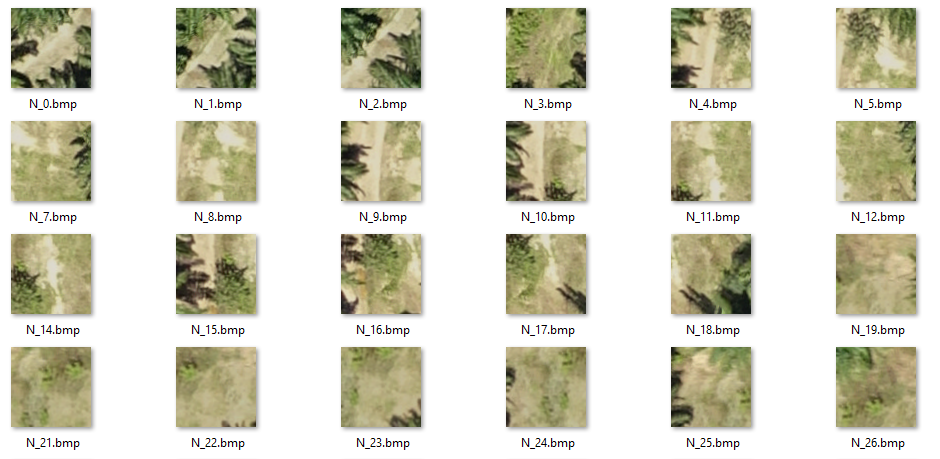
\includegraphics[width=0.9\textwidth]{figures/negativeList.png} % second figure itself
			\caption[Tập ảnh mẫu âm]{Tập ảnh mẫu âm}
		\end{minipage}
	\end{figure}
	\item Cấu hình tham số và chạy máy học Cascade Classifier trong OpenCV. Thư viện OpenCV đã có bộ công cụ giúp luyện một máy học nhận diện đối tượng theo phương pháp của Viola và Jones. Chi tiết về cách sử dụng công cụ này có trong link sau: [docs.opencv.org/3.2.0/dc/d88- -/tutorial\_traincascade.html]. Bộ công cụ này gồm có 3 chương trình chính, chạy trong cửa sổ dòng lệnh:  \textbf{opencv\_createsamples},\\ \textbf{opencv\_traincascade} và \textbf{opencv\_visualisation}.
	\begin{itemize}
		\item Chương trình \textbf{opencv\_createsamples} được sử dụng để đọc dữ liệu mẫu dương, lựa chọn các khung hình có chứa đối tượng cần nhận diện và lưu lại dưới định dạng .vec để sử dụng bởi chương trình \textbf{opencv\_traincascade}.
		\item Chương trình \textbf{opencv\_traincascade} nhận đầu vào là danh sách các dữ liệu mẫu âm, file định dạng .vec được tạo bởi chương trình \textbf{opencv\_createsamples}, và các tham số khác của thuật toán, xuất ra một file mô tả mô hình cascade của máy học nhận dạng, định dạng xml.
		\item File kết quả xml được sử dụng bởi hàm của thư viện OpenCV để tạo ra máy học nhận diện, dựa trên các mô tả và tham số luyện được. Máy học này sẽ nhận đầu vào là ảnh chứa đối tượng cần nhận diện, đâu ra là các khung hình chữ nhật bao quanh đối tượng cần nhận diện.
	\end{itemize}
	\item Hiển thị kết quả thu được từ máy học. Chương trình \textbf{opencv\_visualization} cho phép hiển thị kết quả của quá trình luyện máy học nhận diện cây cọ, là những đặc trưng được lựa chọn, và thứ tự của những đặc trưng này trong máy học phân lớp lên trên một ảnh mẫu cây cọ được chọn.
\begin{figure}[!h]
	\centering
	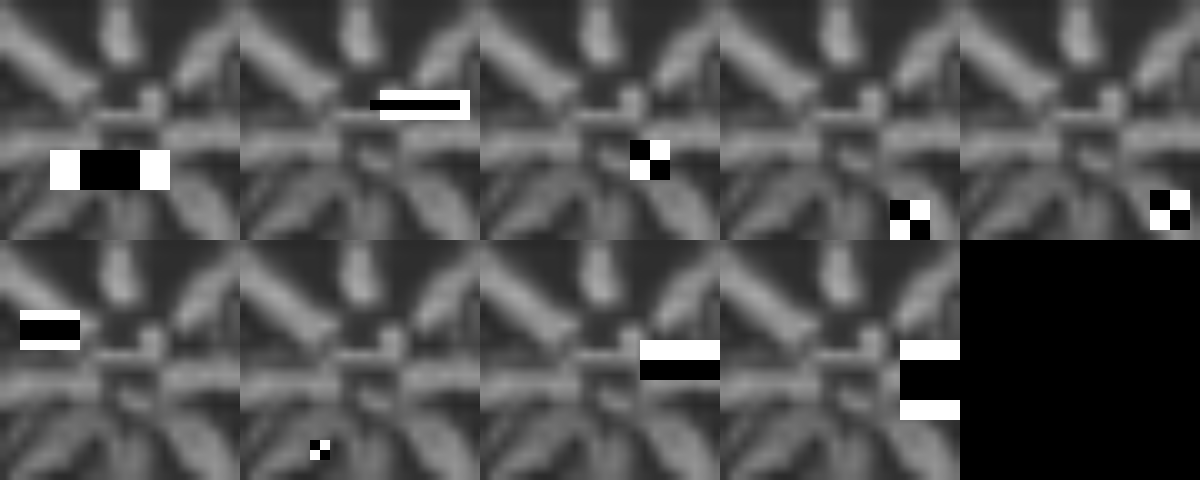
\includegraphics[scale=0.3]{figures/datastage_11.png} 
	\caption[Hiển thị các đặc trưng được lựa chọn của một giai đoạn trong máy học]{Hiển thị các đặc trưng được lựa chọn của một giai đoạn trong máy học.}
\end{figure}	
\end{enumerate}

\subsection{Mô tả chương trình}
Sau khi đã có kết quả của quá trình luyện máy học nhận diện là file xml mô tả máy học và các đặc trưng được lựa chọn, tôi tiếp tục sử dụng thư viện OpenCV, ngôn ngữ lập trình Python và thư viện làm giao diện PySide để xây dựng chương trình desktop cho phép người dùng mở ảnh và chạy thuật toán nhận diện cây cọ với máy học đã được luyện, và lưu kết quả nhận diện dưới dạng file shapefile để dễ dàng sử dụng trong các chương trình hệ thống thông tin địa lý khác như ArcMap hay QGIS.

\begin{figure}[!h]
	\centering
	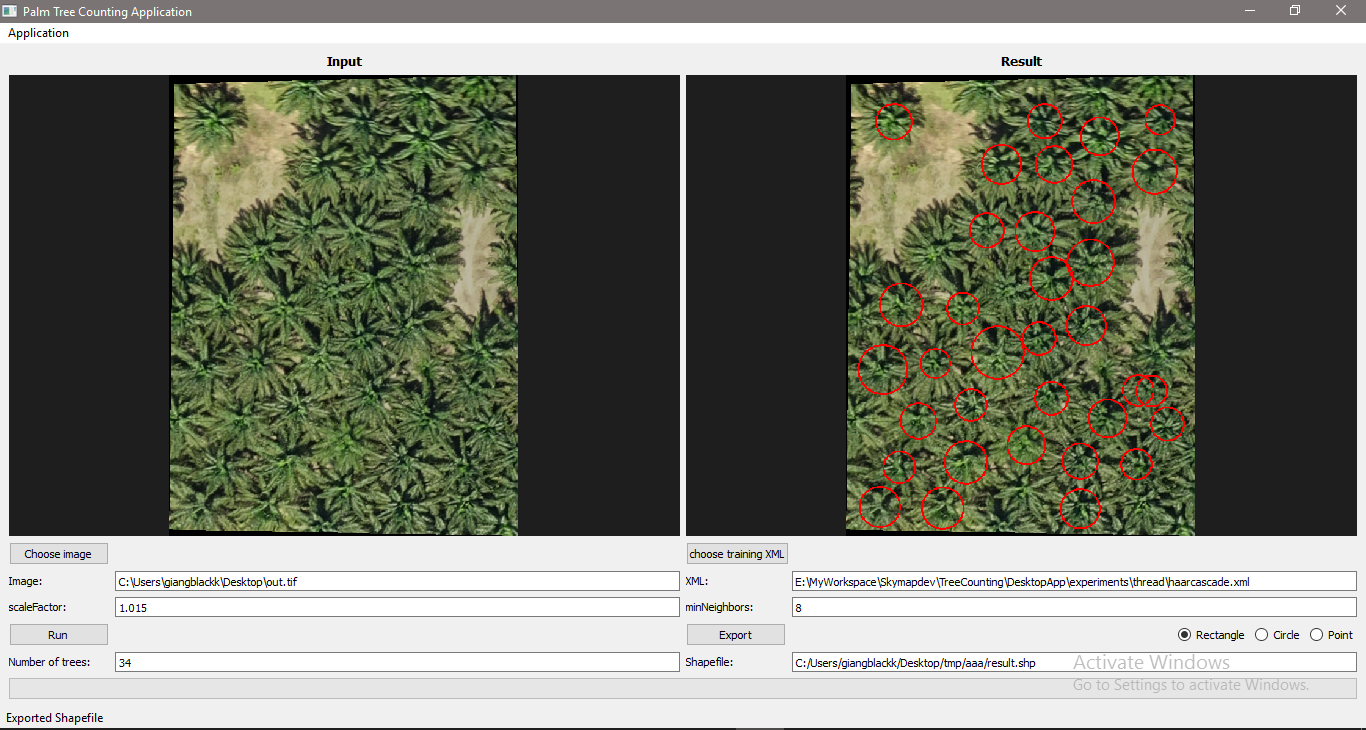
\includegraphics[scale=0.45]{figures/appScreenshot01.png}
	\caption[Giao diện ứng dụng tự động đếm số cây cọ trong ảnh]{Giao diện ứng dụng tự động đếm số cây cọ trong ảnh.}
\end{figure}
\subsection{Kết quả và ước lượng độ chính xác}
Độ chính xác của quá trình nhận dạng được đánh giá định lượng thông qua 3 chỉ số: precision, recall và overall accuracy, được tính dựa trên kết quả nhận diện được khi so sánh với kết quả cây thực sự có trong ảnh.

Công thức của các chỉ số này tham khảo từ [?] như sau:
\begin{equation}
	\text{Precision} = \frac{\text{Số đối tượng nhận diện được đúng là cây cọ}}{\text{Tổng số đối tượng nhận diện}}
\end{equation}
\begin{equation}
	\text{Recall} = \frac{\text{Số đối tượng nhận diện được đúng là cây cọ}}{\text{Số cây cọ thực sự có trong ảnh}}
\end{equation}
\begin{equation}
	\text{Overall Accuracy} = \frac{\text{Precision} + \text{Recall}}{2}
\end{equation}

Một nhận diện được cho là nhận diện đúng cây cọ khi tâm của nhận diện đó cách tâm của một cây cọ thực sự không quá 10 pixel.

Bảng 2 cung cấp kết quả về các chỉ số đánh giá độ chính xác định lượng của chương trình với các dữ liệu mẫu được sử dụng để kiểm tra.

\begin{table}[!h]
	\caption[độ chính xác của các phương pháp trên các dữ liệu kiểm thử]{độ chính xác của các phương pháp trên các dữ liệu kiểm thử}
	\centering
	\begin{tabular}{ |c|c|c|c| } 
		\hline
		Dữ liệu & Precision(\%) & Recall(\%) & Overall Accuracy(\%)\\ 
		\hline
		Vùng 1 & 87.5 & 89.09 & 88.30\\
		Vùng 2 & 96.15 & 89.28 & 92.7\\ 
		Vùng 3 & 94.87 & 82.22 & 88.545\\ 
		Vùng 4 & 90 & 81.81 & 85.9\\ 
		Vùng 5 & 77.78 & 82.35 & 80.06\\ 
		Vùng 6 & 93.33 & 77.78 & 85.56\\ 
		Vùng 7 & 94.53 & 98.25 & 96.39\\ 
		Vùng 8 & 96.96 & 98.76 & 195.72\\ 
		\hline
	\end{tabular}
\end{table}

Ta nhận thấy tỉ lệ chính xác này là tương đối tốt.
\newpage
\section{Kết luận}
Trong báo cáo này, tôi đã trình bày quá trình sử dụng phương pháp nhận diện đối tượng Haar-based Cascade Classifier đề xuất bởi P. Viola và  M. Jones, vào xây dựng máy học nhận diện và đếm số cây cọ trong ảnh viễn thám chất lượng cao thu thập được từ vùng Jalan Bukit Kuantan, Malaysia. Trong quá trình này tôi có sử dụng đến thư viện OpenCV để luyện máy học nhận diện cây cọ và ngôn ngữ lập trình Python, cùng các thư viện mã nguồn mở hỗ trợ xử lý dữ liệu thông tin địa lý khác. Bằng trực quan có thể thấy kết quả của máy học nhận diện vẫn còn chưa đủ tốt, khi có những vùng nhỏ trong ảnh có cây cọ nhưng lại không hề nhận diện được.

Trong những nghiên cứu tiếp theo, tôi đề xuất sử dụng một số hướng giúp cải thiện hiệu quả của phương pháp như: tăng kích thước bộ dữ liệu luyện máy học, gồm có tập dữ liệu có cây cọ và tập dữ liệu không có cây cọ; sử dụng ảnh từ những cây chưa nhận diện được, thêm vào tập dữ liệu luyện để luyện lại; sử dụng các phương pháp máy học khác như convolution neural network.
Do năng lực và thời gian có hạn, báo cáo còn nhiều sai sót mong nhận được góp ý thêm, tôi xin chân thành cảm ơn.
\newpage
%%%%%
\printindex
%%%%%
\newpage
\begin{thebibliography}{9}
	\bibitem{ViolaJones}
	P. Viola and M. Jones,
	\textit{Rapid object detection using a boosted cascade of simple features},
	in IEEE Comp. Soc. Conf. on Computer Vision and Pattern Recognition. CVPR 2001, vol. 1. IEEE, 2001, pp. 1-511.
	\bibitem{indexmundi}
	Palm oil Price, http://www.indexmundi.com/commodities/?commodity=palm-oil
	\bibitem{opencv}
	OpenCV library, http://opencv.org
	\bibitem{cleanmalay}
	Just how Big is Malaysia’s Palm Oil Industry?, http://cleanmalaysia.com/2015/12/09/just-how-big-is-malaysias-palm-oil-industry/
	\bibitem{remotesens}
	Remote Sensing, https://en.wikipedia.org/wiki/Remote\_sensing
	\bibitem{geoeye}
	GeoEye-1 Satellite Image, http://www.satimagingcorp.com/gallery/geoeye-1/
	\bibitem{digiglob}
	Digital Globe, https://www.digitalglobe.com/
	\bibitem{qgis}
	QGIS - A Free and Open Source Geographic Information System, http://www.qgis.org/en/site/
	\bibitem{shapefile}
	Shapefiles, http://doc.arcgis.com/en/arcgis-online/reference/shapefiles.htm
	\bibitem{python}
	Python language, https://www.python.org/
	\bibitem{gdal}
	GDAL - Geospatial Data Abstraction Library, http://gdal.org/
\end{thebibliography}

\end{document}